\chapter{Existence and Absence of Hopf Bifurcation in Phosphorylation–Dephosphorylation CRN}

\section{What even \textbf{is} a bifurcation?}
To better generalise them, it'd be best to also define the notion of:

\begin{definition}
  \textbf{Invariant sets}.

  Taking the Auton. sys.
  \begin{equation}\label{invar_set_auton_sys}
    \dot{y} = f(y) , y(0) = y_0, y \in \mathbb{R}^n
  \end{equation}

  A stateset $S \subseteq \mathbb{R}^n$ of \ref{invar_set_auton_sys} is \textbf{invariant} if $\forall y_0 \in S, \forall t \geq 0: y(t) \in S$
\end{definition}

As you can see by this above definition, equilibria are also particular cases of invariant sets, themselves.

They also fall into stability classes that can be defined as in Def. \ref{equilibrium_stability}, but replacing
\[
  "y_0" \text{ with } "S \subseteq \mathbb{R}^n \text{ }"
\]
and
\[
  " \dotso \norm{y(t) - y_0} \dotso" \text{ with } "\dotso \text{ inf}\{ \norm{y(t) - s} : s \in S  \} \dotso \text{ }"
\]
The Jacobian, generally, would also not be as useful in this context anymore.
\newpage
Now consider we have a system as above, except it now depends on an extra parameter $\mu$, which remains constant \textbf{during} our "experiment".
\begin{equation}\label{auton_parameter_sys_compact}
  \dot{y} = f_\mu(y).
\end{equation}

This could be, for example, the length of the pendulum $L$, in \ref{damped_pendulum}, or its damping coefficient $c$. Honestly generalising it even more, it could even be the gravitational constant $g$. Hence, this parameter can, of course be a \textbf{vector} of such parameters.

The way the parameter $\mu$ varies also induces variations in the topology and dynamics of the system. That's obvious since this is kind of the point of parameters in systems.

What can vary though can be trivial or more intereseting.

The positions of invariant sets, for example can vary continuously

during changes in $\mu$; that's usually normal.

But what's more interesting is when these change their \textbf{stabilty} altogather, equilibria dissapear completely / appear out of thin-air - or, even - collide with other invariant sets.

This odd behaviour is called a \textbf{bifurcation}, and $\mu$, in this case is a \textbf{bifurcation parameter}.

The former types of bifurcations I talked about previously are called \textbf{local}, those in which changes in stabilty can only be considered mostly for \textbf{isolated equilibria}, individually, or other invariant sets whose stabilty can be analysed \textbf{locally}, via the system's linearization at a point.

The latter are \textbf{global}, which are more complex and require greater understanding of the system beyond a local linearization, but that falls into the special-case category described in the last paragraphs of the previous chapter, and so far all I know about Mr. Prof. Lyapunov as of now is his brother was pianist. But thankfully our interest for this work lies with local bifurcations, so we'll be ignoring this for now, maybe I'll come back to it during my Master's (not).

To better define and illustrate them for the 1-D case and give example of bifurcations for such dimension, we could instead write our vector field $f$ as depending on $\mu$ in addition to the unknown function $y$.
\begin{equation}\label{eq:1-d_bif_sys}
  \dot{y} = f(y, \mu).
\end{equation}
And assume $f \in C^k(\mathbb{R} \bigtimes \mathbb{R}), k \geq 2 $ around $(0,0)$, and
\begin{equation}\label{bifurcation_priming}
  f(0,0) = 0, \quad \frac{\partial f}{\partial y}(0,0) = 0.
\end{equation}
By these conditions we are basically "priming" the system for bifurcations, but none are enough for them to actually acuur. Here come the specific definitions for each particular type of bifurcation in 1-D.

\begin{definition}
  A \textbf{Saddle-node bifurcation}:
  for $f$ in \ref{bifurcation_priming}, add as well:
  \begin{equation*}
    \frac{\partial f}{\partial \mu}(0,0) =: a \neq 0, \quad \frac{\partial^2 f}{\partial y^2}(0,0) =:b \neq 0.
  \end{equation*}
\end{definition}
Then, for \ref{eq:1-d_bif_sys}, a saddle-node bifurcation accurs at $\mu = 0$, if the following equivalances are true:

\rom{1}. For $ab < 0$ (resp. $ab> 0$), $\nexists y : f(y,\mu) = 0$ for $\mu < 0$ ( resp. $\mu > 0$)

\rom{2}. For $ab < 0$ (resp. $ab > 0$), $\exists y_+(\epsilon) \neq y_-(\epsilon) \implies y_\pm(\epsilon) : f(y_\pm(\epsilon), \mu) = 0, \epsilon = \sqrt{\abs{\mu}}$, for $ \mu > 0 $ (resp. $\mu < 0$ ), having opposing stabilities.

\begin{definition} \label{pitchfork_bif}
  \textbf{Pitchfork bifurcation}.

  For $f$ from \ref{bifurcation_priming}, assume as well that:
  $f \in C^k, k \geq 3$,
  \[
    f(-y, \mu) = -f(y,\mu)
  \]
  and,
  \[
    \frac{\partial^2 f}{\partial \mu \partial y}(0,0) =: a \neq 0, \quad \frac{\partial^3 f }{\partial y^3}(0,0)=: b \neq 0
  \]

  Now, a \textbf{pitchfork bifurcation} accurs for \ref{eq:1-d_bif_sys} at $\mu  =0$ if:

  \rom{1}. for $ab < 0$ (resp. $ab > 0$) $\exists! y = 0 :f(y,\mu) = 0 $ for $\mu < 0$ (resp. $\mu > 0$). $b < 0 \implies$ stable, $b > 0 \implies$ unstable.

  \rom{2}. for $ab < 0$ (resp. $ab > 0$) $\exists y = 0 : f(y , \mu) = 0$, as well as: $y_+(\epsilon) \neq y_-(\epsilon) \implies y_\pm(\epsilon) : f(y_\pm(\epsilon), \mu) = 0, \epsilon = \sqrt{\abs{\mu}}$  for $\mu > 0$ (resp. $\mu < 0$), for which $y_+(\epsilon) = -y_-(\epsilon)$, Both $y_-(\epsilon)$ and $y_+(\epsilon)$ have matching stabilities, whereas $y = 0$ has the opposite stability of them, given by $b < 0 \implies$ stable, $b > 0 \implies$ unstable.
\end{definition}

\begin{definition}
  \textbf{Transcritical bifurcation}.

  For $f$ in \ref{bifurcation_priming}:
  \[
    \frac{\partial^2 f}{\partial \mu \partial y}(0, 0) =:a \neq 0, \quad \frac{\partial^2 f}{\partial y^2}(0,0) =: b \neq 0
  \]
  Then a \textbf{transcritical bifurcation} accurs for \ref{eq:1-d_bif_sys} at $\mu = 0$, char. by (if they hold):

  \rom{1}.  $\exists y = 0 : f(y, \mu) = 0$  and  $ \exists y_0(\mu) : f(y_0(\mu), \mu) = 0 $ where $\mu \rightarrow u_0(\mu) \in C^m, m = k - 2$

  \rom{2}.  for $a\mu  < 0$ (resp. $a\mu > 0$) the trivial fixed point $y = 0 \implies$ stable (resp. unstable)
  and $u_0(\mu)$ has opposing stability.
\end{definition}

Finding local bifurcations can be done by looking at eigenvalues.
\newpage
{\large The local bifurcation condition

}For system:
\begin{equation}
  \dot{y} = f(y, \mu) \quad f : \mathbb{R}^n \times \mathbb{R} \rightarrow \mathbb{R}^n
\end{equation}

\begin{definition}\label{local_bif_def}
  $(y_0,\mu_0)$ admits a \textbf{local bifurcation} if:
\end{definition}

If $\forall \lambda \in Eig(J_{f}(y_0,\mu_0)) : Re(\lambda) \leq 0$, while $\exists \lambda_0 : Re(\lambda_0) = 0$

\begin{equation}\label{stable_state_bif}
  \text{If } \lambda_0 = 0 \text{ the bifurcation is stable-state defined. }
\end{equation}

We also have a second kind of local bifurcation and this is where we begin the crux of the thesis, and answear the first question I had getting into this:

\section{What is a simple Hopf Bifurcation?}

A \textit{simple Hopf bifurcation} is a bifurcation in which a single complex-conjugate pair of eigenvalues of the Jacobian matrix crosses the imaginary axis, while all other eigenvalues remain with negative real parts. Such a bifurcation generates nearby oscillations or periodic orbits.

Or, more formally, defined in a simmilar fashion to Def. \ref{local_bif_def}:

\newpage
\begin{definition}
  $(y_0, \mu_0)$ admits a \textbf{Hopf bifurcation} if we have Def. \ref{local_bif_def}, and additionally:
  \begin{equation}\label{hopf_bif_def}
    \exists! \lambda_0 : Re(\lambda_0) = 0, \quad
    Im(\lambda_0) \neq 0.
  \end{equation}
\end{definition}
Visually, just to hammer it in:

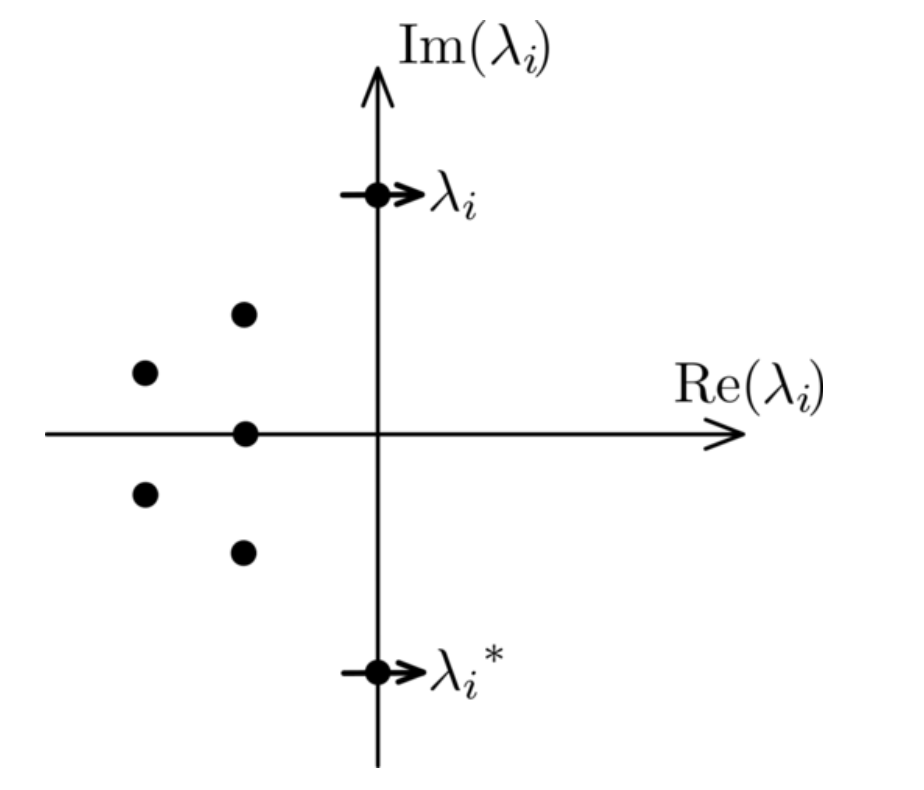
\includegraphics[width=13cm]{math_pics/hopf-bif-eigenvalue-graph.png}

In $\mathbb{R}^2$, such Bifurcations cause special kinds of invariant sets, namely \textbf{limit cycles} to appear. These are periodic solutions, for which we'll need a few more concepts in order to be able to define them:
\begin{definition} \textbf{Closed trajectory and Closed orbit (cycle)}

  A trajectory (or flow): $y(t) \in \mathbb{R}^2$ as in Def. \ref{dyn_sys_orbit_flow_etc_def} is a solution for \ref{eq:1-d_bif_sys}

  A closed trajectory is one which returns to its starting point $\forall s_0 := \Phi(0,s) $ it has, namely:
  \begin{gather*}
    \exists t_0 \in T : \Phi(t,s) = \Phi(t+t_0,s), \forall s \in \Phi_{s_0}     \\
    \Updownarrow \\
    \exists t_0 \in T : y(t) = y(t+t_0), \forall t \in T
  \end{gather*}
  A \textbf{closed orbit} or \textbf{cycle} is just the image of such a closed trajectory.
\end{definition}

\begin{definition}\textbf{Limit point}
  These can be grouped into $\omega$ (attracting) and $\alpha$ (repelling) limit points:

  $y_\omega$ is an $\omega$-limit point  for $y$ if:

  $\exists (t_n)_{n \in \mathbb{N}} \subseteq I(y) : $
  \begin{gather*}
    \lim_{n \rightarrow \infty} t_n = \infty  \\
    \lim_{n \rightarrow \infty} \Phi(t_n,y) = y_\omega
  \end{gather*}
  And similarly, but in reverse:

  $y_\alpha$ is an $\alpha$-limit point  for $y$ if:

  $\exists (t_n)_{n \in \mathbb{N}} \subseteq I(y) : $
  \begin{gather*}
    \lim_{n \rightarrow \infty} t_n = \textbf{--} \infty  \\
    \lim_{n \rightarrow \infty} \Phi(t_n,y) = y_\alpha
  \end{gather*}
\end{definition}

\begin{definition}\textbf{Limit set}
  The set of all $\omega$ (or $\alpha$)-limit points for a particular orbit $\gamma$ is called the \textbf{limit set} of $\gamma$, denoted and defined as:
  \[
    \lim_{\omega}\gamma_s := \bigcap_{t \in T} \overline{ \{ \Phi(t', s) : t' > t \} }
  \]
  \[
    \lim_{\alpha}\gamma_s := \bigcap_{t \in T} \overline{ \{ \Phi(t', s) : t' < t \} }
  \]
\end{definition}

\begin{definition} \textbf{Limit cycle}

  A Limit Cycle is a cycle which is the limit set of at least another trajectory.
  Also, interestingly:
  \[
    \lim_{\omega}\gamma \bigcap \gamma  = \emptyset \implies \text{ it's an } \omega \text{-limit cycle}.
  \]
  \[
    \lim_{\alpha}\gamma \bigcap \gamma  = \emptyset \implies \text{ it's an } \alpha \text{-limit cycle}.
  \]
\end{definition}

//TODO: Proof: trust me bro;

What's interesting though, and makes calculations easier for the 2-D case is:
\begin{theorem}  \textbf{Poincare-Bendixson}

  //TODO afla cu msa-i scrii numele real fara sa dea latexu eroare gen poincare cu o ghilimea din aia deaspura la r

  For a dynamical system $(T,X,\Phi)$ with $X \subseteq \mathbb{R}^2$, $\forall$ compact invariant set $S$.
  \begin{gather*}
    \text{if } \nexists x_0 \in S : \Phi(t_1, x_0) = \Phi(t_2,x_0), \forall t_1,t_2 \in T \\
    \Downarrow \\
    \forall s \in S: \gamma_s \text{ are either limit cycles, or } \lim_{\omega / \alpha}\gamma_s \text{ is a $\omega$ (or $\alpha$)-limit cycle }.
  \end{gather*}
\end{theorem}

But the problem is this theorem only holds for $\mathbb{R}^2$. For higher dimensions we don't have this property necessarily, instead we have to look for periodic solutions (limit cycles) ourselves - which, as stated previously - accur naturally during a Hopf bifurcation.

So having these in mind, Hopf is kind of like a $\mathbb{R}^n$ version of Pitchfork bif.: \ref{pitchfork_bif} when you think about it.

//TODO: scrie (si fa mai mult research) despre  \textbf{normal form} si despre cum aproximeaza el sistemul dinamic in jurul punctelor de bifurcatie, ca o sa-ti fie de folos la cam toate punctele de birufcatie sincer pare important si chiarn u stiu de el am vzt in mai multe parti
//TODO: sincer mai bine lasa tbh noone cares as of now

\subsection{Proving the existence of simple Hopf bifurcations}

For this sub-chapter we would first need to define (and show how to obtain) one of the most important tools in this study: the Hurwitz matrix and its determinants.

The english mathematician Edward John Routh was looking at the (\ref{eq:lin_approx}) of
\[
  x_i' = f_i(x_1,\dots , x_n), \quad i = \overline{1,n}
\]
Namely:
\[
  x_i' =\sum_{j=1}^{n}a_{ij} x_j, \quad a_{ij} = \frac{\partial f_i}{\partial x_j}(0)
\]
But he figured out he doesn't have to find the roots of
\begin{equation}\label{lin_apporx_char_equation}
  det(J - \lambda I_n) = a_0 \lambda^n + a_1 \lambda^{n-1} + \dots + a_{n-1}\lambda + a_n = 0
  3k
\end{equation}
To infer the system's stability, as in check:
\[
  Re(\lambda_0) \leq 0
\]
but can instead instead just simply look at the coefficients of \ref{lin_apporx_char_equation}: $a_{i}$ to verify it.

To do this he used:

\rom{1}: Cauchy's argument principle

and

\rom{2}: Sturm's theorem

\rom{1}

Cauchy's argument principle states that for the poly. $p \in \mathbb{C}[Z]$:
\[
  p(z) = u(z) + i v(z), \quad u, v \in \mathbb{R}[Z]; u,v : \mathbb{C} \rightarrow \mathbb{R}
\]
Its number of roots inside a closed contour $\gamma$  is $=$ to the number of positive rotations (counter-clockwise)[c.c.] that $(u(z), v(z))$ (or $arg(p(z))$) makes as $z$ moves across $\partial \gamma$ in a positive sense [c.c.].

//TODO: ai putea sa pui si tu o poza cu un vector space format de un anumit polinom complex cu valori complexe

Now all we need to do is make this "closed contour" the entire left-half of the complex axis!

We could write it as a {\large HUGE} half-circle
\[
  z = Re^{i \theta}, \quad \frac{\pi}{2} \leq \theta \leq \frac{3 \pi}{2}, R \text{ sufficiently large }
\]

The thing is even if it's the case that all $n$ roots lie inside it, $arg(p(z))$ will only make $\frac{n}{2}$ rotations since this is a half circle, so we could combine this fact with a more elegant way of writing "the half-plane, left of the imaginary axis" into:

\begin{lemma}\label{cauchy_arg_lemma}
  For $p(z) \in \mathbb{C}_n[Z]$ and $p(ix) \neq 0. \forall x \in \mathbb{R}$. Then $\forall z_0 : p(z_0) = 0, Re(z_0) < 0 \iff$ $arg(p(ix))$ makes $\frac{n}{2}$ positive rotations for $x \in [-\infty , \infty]$.
\end{lemma}

\rom{2}.

The second tool he's used was Sturm's theorem, which was the result of his discovery that for the division $\frac{p_{i-1}(x)}{p_i(x)}$, for $p_k \in \mathbb{R}[X]$ it's better to take the remainder $p_{i+1}(x)$ with a negative sign:
\begin{equation}\label{euclid_algorithm}
  p_{i-1}(x) = p_i(x) q_i(x) - p_{i+1}(x) \tag{Euclid's Algorithm}
\end{equation}
Because, if we do that, then:
\begin{equation}\label{sturm_seq_property}
  \text{sign} ( p_{i+1}(x) )  \neq \text{sign} ( p_{i-1}(x) ), \quad \text{for} \quad p_i(x)=0 \tag{Sturm. Seq. Property}
\end{equation}
This is called the "Sturm sequence property"

And if we construct a sequence
\[
  (p_k)_{k = \overline{0,m}} \subset \mathbb{R}[X]
\]
and the function
\begin{gather}\label{no_sign_changes_func}
  w : \mathbb{R} \rightarrow \mathbb{R} \notag  \\
  w(x) = \text{No. of sign changes of  } (p_k)(x) \notag
\end{gather}
Then we find that for:
\begin{gather*}
  p_i^{-1}(0) \text{ ( set of roots for $p_i$) } \\
  R := \bigcup_{i \in \left\{ 1, \dots, m-1 \right\} } p_i^{-1}(0) \\
  \forall x_1, x_2 \in R, w(x_1) = w(x_2)
\end{gather*}
Hence we have:
\begin{lemma}\label{sturm_lemma}
  For a seq. of $  (p_k)_{k = \overline{0,m}} \subset \mathbb{R}[X]$ that satifies:

\rom{1})
$ deg(p_0) > deg(p_1), $

\rom{2})
$\nexists x \in \mathbb{R} : p_0(x) = p_1(x) = 0, $

\rom{3})
$p_m(x) \neq 0, \forall x \in \mathbb{R}$

\rom{4})
And (\ref{sturm_seq_property})
\par
We have (for the above defined $w$ \ref{no_sign_changes_func}) :
\begin{gather}
\frac{w(\infty) - w(-\infty)}{2} =  \notag \\
\text{No. of positive rotations of the vector } \notag \\
(p_0(x), p_1(x)), \text{as $x$ tends from  } x \in [-\infty, +\infty] \notag
\end{gather}
\end{lemma}

Proof:

As stated in \ref{sturm_seq_property}: $w(x)$ doesn't change at roots of

$p_k(x), k = \overline{1,m-1}$. Asumption \rom{3}) shows $p_m(x)$ doesn't influence it either. So there can only be one suspect: $p_0(x)$. If there's a spike by $1$ at $\overline{x}$, zero of $p_0$ (   $p_0(\overline{x}) =0 $) either:
\[
p_0(x) \text{changes from + to - and   } p_1(\overline{x}) > 0
\]
or:
\[
p_0(x) \text{changes from - to + and  } p_1(\overline{x}) < 0
\]
[   $\nexists \overline{x}: p_1(\overline{x}) = 0$ by assumption \rom{2})  ]

Both of which cause the vector $(p_0(x), p_1(x))$ to cross the imaginary axis in a positive sense.

If there's a dip of $w$ at $\overline{x}$, however, the crossing is done clock-wise, this time.

Now taking \rom{1}) into account and the fact that $(p_0(y), p_1(y))$ is horizontal for $y \rightarrow  - \infty$ and $y \rightarrow + \infty  $ outcomes the result of our lemma
\qed

//TODO Maybe try to draw this yourself cu arrows nstuff

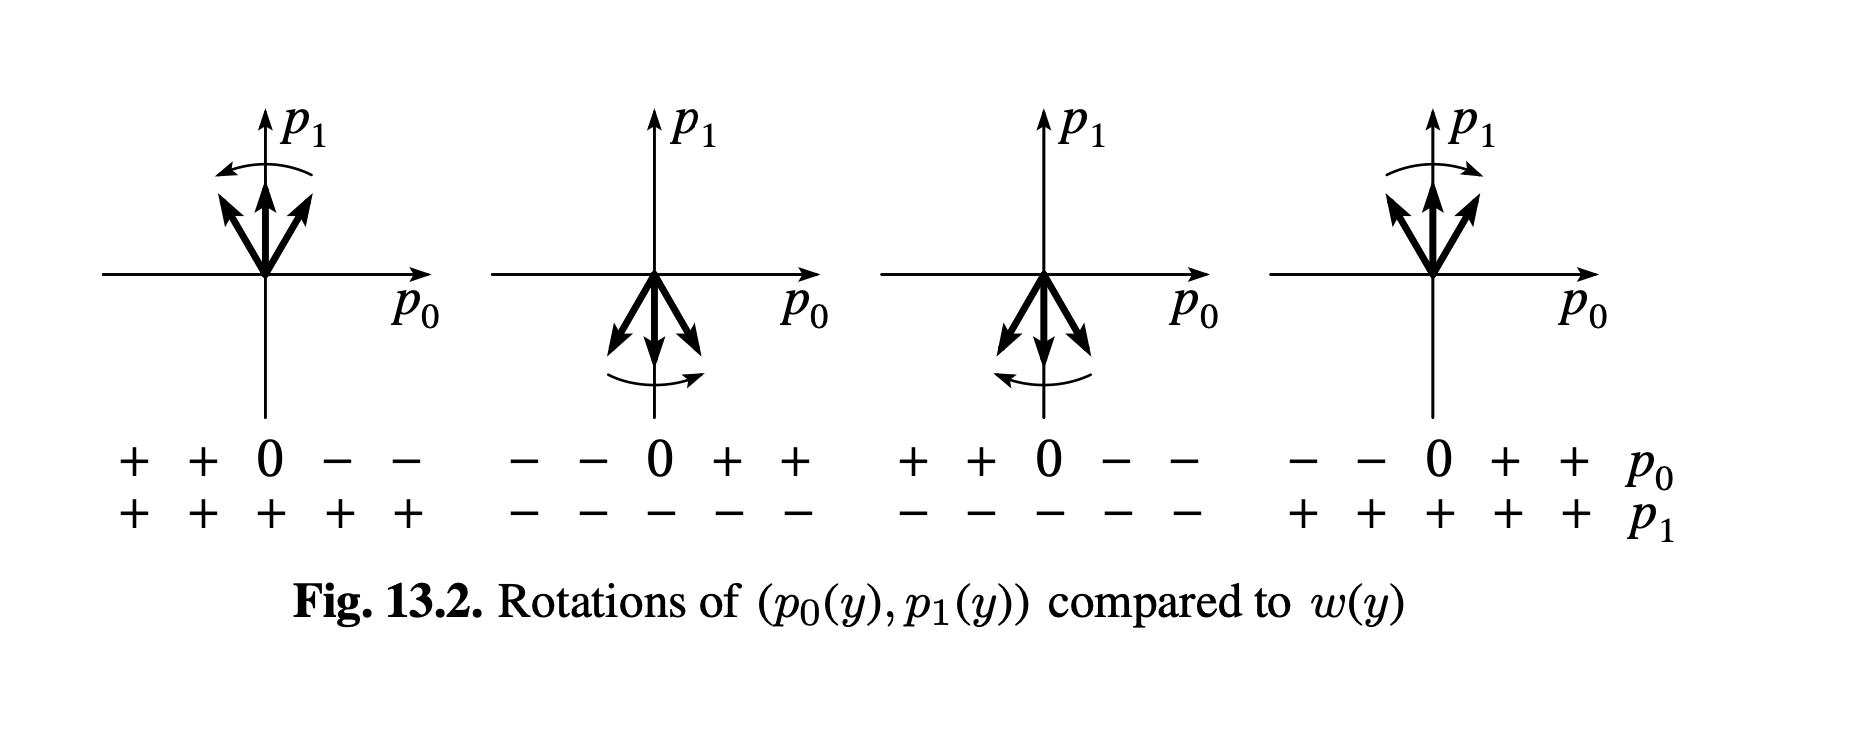
\includegraphics[width=13cm]{math_pics/sageti-cumse-invart.png}

So using these 2 Lemmas we have the criteria for stabilty:
For the characteristic polynomial \ref{lin_apporx_char_equation}, written instead like this:
\[
p(z)=a_0 z^n + a_1z^{n-1} + \dots + a_n = 0, \quad a_0 > 0
\]

Dividing $\frac{p(i x)}{i^n}$ and using \ref{real_imag_another_way_to_write}

\begin{gather}
p_0(x)= \text{Re}(\frac{p(i x)}{i^n}) = a_0 x^{n} -a_2 x^{n-2} + a_4 x^{n-4} \pm \dots \\
p_1(x)= -\text{Im} (\frac{p(i x)}{i^n}) = a_1 x^{n-1} -a_3 x^{n-3} + a_5 x^{n-5} \pm \dots
\end{gather}

More generally:
\begin{equation}\label{polys_general_form}
p_i(x) = c_{i0} x^{n-i} + c_{i1} x^{n-i-2} + c_{ i2 } x^{ n-i-4  } + \dots, \tag{Gen. Form}
\end{equation}

And $q_i(x) = (  \frac{c_{ i-1 ,0}}{c_{ i0 }} )x$ from \ref{euclid_algorithm} given that $c_{i0} \neq 0$.
Putting \ref{polys_general_form} into \ref{euclid_algorithm} to get the general form of all the coefficients as well we get:
\begin{align}\label{coeff_gen_form}
c_{i+1,j} = c_{i,j+1} \cdot \frac{c_{i-1,0}}{c_{i,0}} - c_{i-1,j+1 } = \frac{1}{c_{i,0}} \text{det}
\begin{pmatrix}
c_{i-1,0} & c_{i-1, j+1} \\
c_{i,0} & c_{i, j+1} \tag{Coeff.}
\end{pmatrix}
\end{align}

The algo. stops for $ p_m(x) $ with $ m < n$ if $c_{i,0} = 0$ at a particular $i \implies q_i(x)$ is of higher degree.

And so: $(p_i(x))_{i = \overline{1,m \text{ or } n}}$ verifies \rom{1}), \rom{4}) from \ref{sturm_lemma}

\rom{2}) $\iff p(ix) \neq 0, \forall x \in \mathbb{R}$

$p_m(x) = \text{gcd}(p_0(x), p_1(x)) \iff \text{ \rom{2}) } \implies \text{ \rom{3}) }$

\par

So here's the big guy:

\begin{theorem}\label{routh_theorem}
(Routh 1877).
\begin{gather*}
Re(\lambda) < 0, \quad \forall \lambda \in \text{det}(J - \lambda I_n)^{-1}(0) \text{ from \ref{lin_apporx_char_equation} with } a_0 > 0 \\
\Updownarrow  \\
c_{i,0} > 0 \forall,  i = \overline{1,n}
\end{gather*}
\end{theorem}

\textbf{Proof: } $arg(p_0,p_1) = 360^\degree - arg(\text{Re}(p), \text{Im}(p)) \implies \frac{n}{2}$ positive rotations of $p(ix)$ are bascially $\frac{n}{2}$ neg. rot. of $(p_0(x), p_1(x))$. If $Re(\lambda) < 0, \forall \lambda \in p(\lambda)^{-1}(0) \implies$ ( from  \ref{cauchy_arg_lemma}, \ref{sturm_lemma} ) $w(\infty) - w( - \infty) = -n$. Could only be for $w(\infty) = 0, w(- \infty) = n$, though. $ \implies p_i(x) \geq 0$ for all leading $i$. Having \ref{routh_theorem} $\implies p_n(x) \equiv c_{n0}$. Because $\nexists \text{gcd}(p_0(x),p_1(x)), p(\lambda) \neq 0$ for Re$(\lambda) = 0$. Now we just do \ref{cauchy_arg_lemma} + \ref{sturm_lemma} once more. \qed

\subsection{Ruling out simple Hopf bifurcations}

\subsection{Convex parameters}

\section{What is a Phosphorylation–Dephosphorylation CRN?}

\subsection{Cyclic and mixed distributive and processive Phosphorylation–Dephosphorylation CRN}